\begin{figure}[h]
    \centering
    \vspace{-10pt}
    \captionsetup{font=small}
    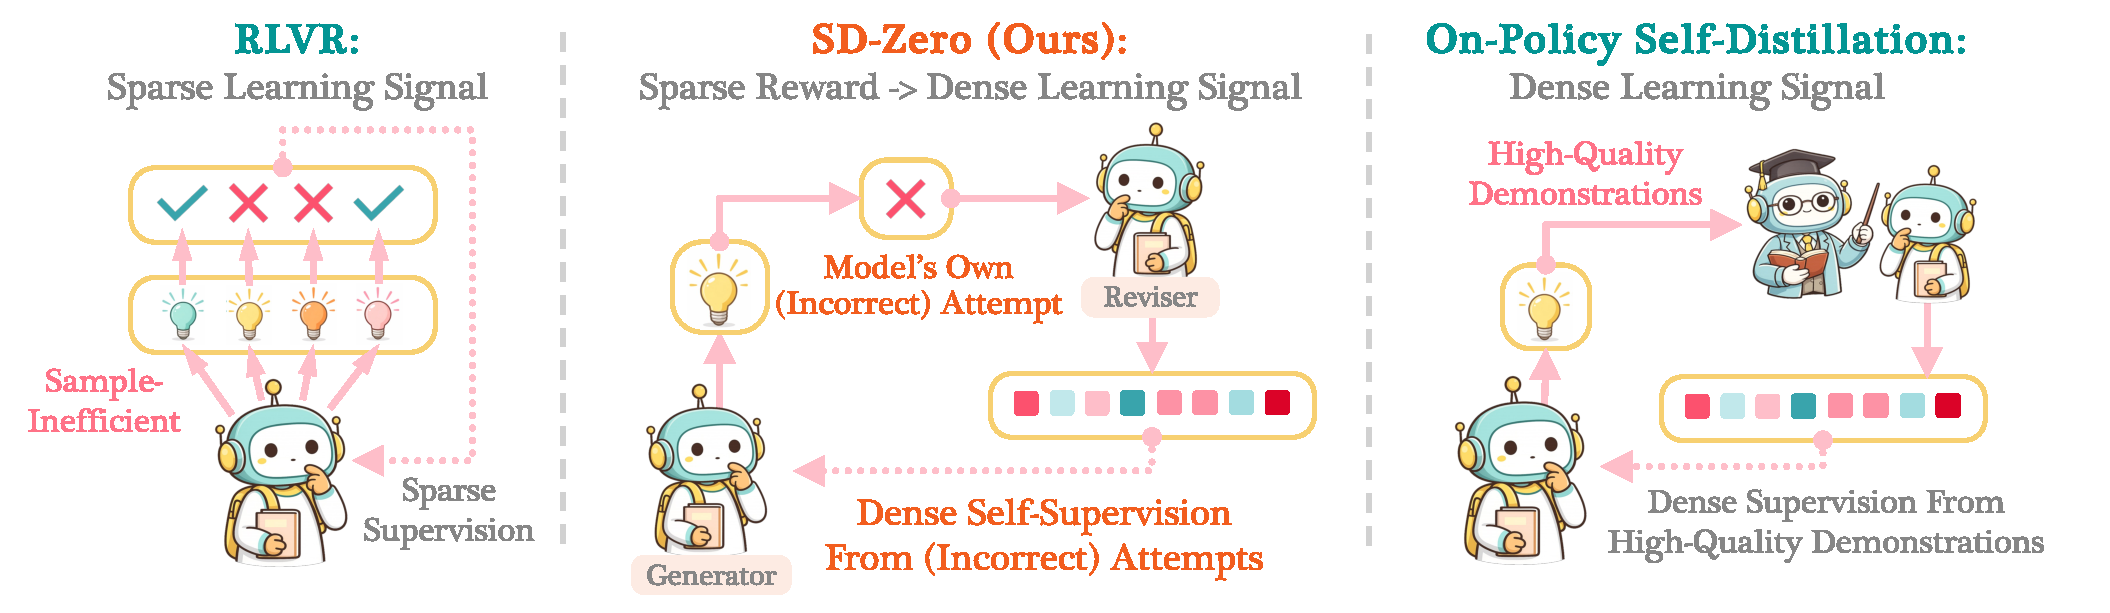
\includegraphics[width=0.95\textwidth]{figures/Picture0.pdf}
    \vspace{-5pt}
    \caption{
    % Reinforcement learning from verified rewards (RLVR) provides sparse learning signals; on-policy distillation relies on an external teacher to provide dense supervision. 
    We introduce \textbf{\ours{}}, an on-policy self-distillation paradigm where the teacher (\emph{reviser}) can condition on incorrect student (\emph{generator}) attempts.
    % that 
    % converts sparse rewards into dense self-supervision through self-revision feedback, without relying on high-quality demonstrations.
    % \danqi{This is my biggest confusion. This figure is about how self-distillation is different from RLVR and onpodi, but not about how your method is different from other self-distillation methods. There is no generator or reviser in the figure.}
    }
    \label{fig:starter}
\end{figure}